\section{Methodology}

\subsection{Study Area and Data}
All parcel, climate, soil, price and yield inputs come from public sources.
Parcels are OpenStreetMap land-use polygons~\cite{osm}. Of 941 polygons, 316
have a centroid in the West Bank. These were classified with the OCHA
administrative layer~\cite{ocha}, restricted to the class under Palestinian
administration, and filtered to 0.1--100\,ha, leaving 174 parcels covering
1{,}464\,ha (Fig.~\ref{fig:map}).

\begin{figure}[t]
\centering
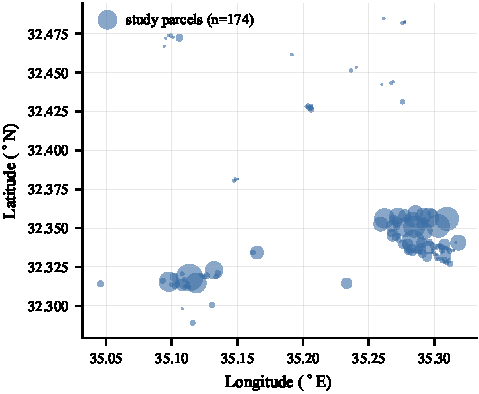
\includegraphics[width=0.92\columnwidth]{figures/fig_map.pdf}
\caption{The 174 study parcels in Jenin governorate.}
\label{fig:map}
\end{figure}

Monthly NASA POWER data for 2015--2024~\cite{nasapower} give 465\,mm of
annual rainfall (90\% in November--March), 20.7\,$^\circ$C and 68.7\%
relative humidity. The governorate is a single grid cell, so climate is the
same for every parcel. Soil properties are SoilGrids 250\,m
estimates~\cite{poggio2021} for 149 of the parcels; the other 25 take the
governorate mean.

Prices are FAOSTAT producer means for 2019--2023~\cite{faostat}. The year
2024 was left out because perishable prices rose 1.24--5.76-fold over 2023
while wheat (0.95) and olives (1.10) did not, indicating a wartime supply
shock. Yields are FAOSTAT means for
2014--2022. National vegetable yields include greenhouse production, so
vegetables and maize were scaled jointly to a mean of 19.65\,t/ha, the PCBS
open-field level for the northern West Bank~\cite{pcbs}, and tree crops by
the factor that brings olives to 1.43\,t/ha. Net irrigation needs follow
FAO-56~\cite{allen1998}. Production cost is an assumed fraction of baseline
gross revenue for each production system, held fixed when prices vary
(Table~\ref{tab:crops}). The water budget is the 1.0\,Mm$^3$/yr of licensed
agricultural abstraction reported by PCBS~\cite{pcbswater}.

\begin{table}[t]
\centering
\caption{Parameters of the ten study crops}
\label{tab:crops}
\footnotesize
\begin{tabular}{lrrrr}
\toprule
 & Price & Yield & Net irrigation & Cost \\
Crop & (USD/t) & (t/ha) & (m$^3$/ha) & (\% of revenue) \\
\midrule
Wheat     &  568 &  2.41 &  500 & 65 \\
Maize     &  572 &  5.79 & 5000 & 65 \\
\midrule
Potatoes  &  488 & 13.27 & 4000 & 55 \\
Tomatoes  &  628 & 51.74 & 6000 & 55 \\
Cucumbers &  614 & 18.49 & 4500 & 55 \\
Onions    &  526 &  9.56 & 3500 & 55 \\
Eggplants &  459 & 19.04 & 6000 & 55 \\
\midrule
Olives    & 1752 &  1.43 & 1500 & 40 \\
Grapes    &  987 &  9.38 & 3000 & 40 \\
Oranges   &  601 & 19.38 & 7000 & 40 \\
\bottomrule
\end{tabular}
\end{table}

\subsection{Suitability Model}
A 300-tree Random Forest~\cite{breiman2001} was trained on N, P, K,
temperature, humidity, pH and rainfall. The real data are 1{,}900 labelled
samples over 19 crops from a public dataset~\cite{kagglecrop}, after its
maize, grape and orange rows were removed. A further 1{,}000 synthetic
samples, generated from FAO EcoCrop envelopes~\cite{ecocrop}, label all ten
study crops. The two sources are evaluated separately. For crop $j$ on
parcel $i$,
\begin{equation}
s_{ij} = \mathrm{RF}_j(\mathbf{x}_{ij})\,\phi(\ell_i, j),
\label{eq:suit}
\end{equation}
where $\mathbf{x}_{ij}$ holds the parcel's soil and climate with the
rainfall feature set to annual rainfall plus the irrigation of crop $j$,
$\mathrm{RF}_j$ is the unnormalised class probability, and $\phi$ weights
the OSM class $\ell_i$: 0.9 for tree crops and 0.3 for annuals on orchards
and vineyards, and 0.9 for annuals and 0.35 for tree crops elsewhere. P and
K have no parcel-level source and were drawn from published ranges in 200
Monte Carlo samples, giving $s_{ij}$ a mean standard deviation of 0.025.
Available N is an assumed 2\% of SoilGrids total N. A pair is unsuitable if
its probability is zero or fewer than 20\% of parcels score at or below
it for crop $j$; with heavy ties, this marks 96 of 1{,}740 pairs.

\subsection{QUBO Formulation}
The binary $x_{ij}$ equals 1 when parcel $i$ grows crop $j$, with $j=0$ for
fallow. With parcel area $a_i$ and yield $y_j$, supply is
$Q_j = \sum_i a_i y_j x_{ij}$, and the plan maximises
\begin{equation}
\sum_j \left( p_j Q_j - \beta_j Q_j^2 \right)
- \sum_{i,j} \left( c_j + \lambda w_j \right) a_i x_{ij},
\label{eq:objective}
\end{equation}
where $p_j$ is the price, $c_j$ the cost and $w_j$ the net irrigation per
hectare, and $\lambda = 0.15$\,USD/m$^3$ unless swept. With
$\beta_j = p_j/(2D_j)$, price falls linearly with supply and crop revenue
peaks at $Q_j = D_j$. The $Q_j^2$ term couples all parcels sharing a crop
into ten 174-node cliques. No crop-level demand data exist for Jenin, so market size is an
assumption, $D_j = 0.6\,A\,y_j$ with $A$ the total study area, kept fixed
across counterfactuals. For the solvers, the negated objective is
divided by its largest linear coefficient, and penalties of weight $M = 0.5$
are added for parcels without exactly one crop and for unsuitable pairs.
Profit is recomputed in USD from each decoded plan, without the water
charge.

\subsection{Encodings and Solvers}
\textbf{One-hot} encoding uses $C = 11$ binaries per parcel with the penalty
$M(\sum_j x_{ij} - 1)^2$, giving 1{,}914 variables; parcels with zero or
several crops remain reachable. \textbf{Domain-wall}
encoding~\cite{chancellor2019} uses $C-1 = 10$ binaries $d_{ij}$ per
parcel, kept non-increasing in $j$ by an ordering penalty of weight
$M_{\mathrm{wall}}$, and reads $x_{ij} = d_{ij} - d_{i,j+1}$ with
$d_{i0} = 1$ and $d_{iC} = 0$ (1{,}740 variables). It replaces the one-crop penalty with this ordering penalty and retains the
suitability penalty, so the two encodings pose the same allocation problem but
not the same penalty landscape; Section~\ref{sec:results} measures how much
that distinction costs. Decoding takes a
one-hot block's lowest-indexed active option (fallow if none) and reads a
domain-wall chain up to its first zero; invalid parcels are counted before
decoding. The main
benchmark uses $M_{\mathrm{wall}} = 1$; Section~\ref{sec:results} also
sweeps $M_{\mathrm{wall}} \in \{0.25, 0.5, 1, 2, 4\}$.

\textbf{SA}~\cite{kirkpatrick1983} flips single bits with $O(n)$
incremental energy updates and cools geometrically from
$T_0 = 0.5\,\mathrm{mean}_i \sum_k |Q_{ik}|$ to $10^{-4}T_0$.
\textbf{dSB}~\cite{goto2021} evolves positions $x_i$ and momenta $y_i$ as
\begin{equation}
\begin{aligned}
\dot{y}_i &= -\left(a_0 - p(t)\right) x_i
- c_0 \Big( \sum_k J_{ik}\,\mathrm{sgn}(x_k) + h_i \Big),\\
\dot{x}_i &= a_0 y_i,
\end{aligned}
\label{eq:dsb}
\end{equation}
where $J$ and $h$ are the Ising couplings and fields, with inelastic walls
at $|x_i| = 1$, $a_0 = 1$, a linearly rising pump $p(t)$, step 0.25 and
$c_0 = 0.5/(\sqrt{N}\,\sigma_J)$. Both solvers return the lowest-energy
state visited; dSB evaluates its sign state every 50 steps and at the end.
\textbf{Greedy} gives each parcel its highest-margin suitable crop, ignoring
market coupling. The Budget column of Table~\ref{tab:bench} reports profit
after fallowing parcels of every plan, greedy included, in ascending margin
per m$^3$ until the water budget is met; other profits precede this repair.

\textbf{Protocol.} Following benchmarking practice for stochastic
solvers~\cite{beiranvand2017}, each arm received a fixed wall-clock budget
of 2.5\,s
per run, which corresponds to 2{,}934 and 4{,}313 dSB steps and 270 and 249
SA sweeps on the one-hot and domain-wall matrices. Arms whose median
time deviated by over 12\% were re-run, and results were rejected beyond
15\%. Each arm used 20 independent seeds, compared by two-sided
Mann--Whitney $U$ tests.
